\documentclass[journal,12pt,twocolumn]{IEEEtran}
%
\usepackage{setspace}
\usepackage{gensymb}
%\doublespacing
\singlespacing

%\usepackage{graphicx}
%\usepackage{amssymb}
%\usepackage{relsize}
\usepackage[cmex10]{amsmath}
%\usepackage{amsthm}
%\interdisplaylinepenalty=2500
%\savesymbol{iint}
%\usepackage{txfonts}
%\restoresymbol{TXF}{iint}
%\usepackage{wasysym}
\usepackage{amsthm}
%\usepackage{iithtlc}
\usepackage{mathrsfs}
\usepackage{txfonts}
\usepackage{stfloats}
\usepackage{bm}
\usepackage{cite}
\usepackage{cases}
\usepackage{subfig}
%\usepackage{xtab}
\usepackage{longtable}
\usepackage{multirow}
%\usepackage{algorithm}
%\usepackage{algpseudocode}
\usepackage[utf8]{inputenc}
\usepackage{tikz}
\usetikzlibrary{positioning}
\usepackage{enumitem}
\usepackage{mathtools}
\usepackage{steinmetz}
\usepackage{tikz}
\usepackage{circuitikz}
\usepackage{verbatim}
\usepackage{tfrupee}
\usepackage[breaklinks=true]{hyperref}
%\usepackage{stmaryrd}
\usepackage{tkz-euclide} % loads  TikZ and tkz-base
%\usetkzobj{all}
\usetikzlibrary{calc,math}
\usepackage{listings}
    \usepackage{color}                                            %%
    \usepackage{array}                                            %%
    \usepackage{longtable}                                        %%
    \usepackage{calc}                                             %%
    \usepackage{multirow}                                         %%
    \usepackage{hhline}                                           %%
    \usepackage{ifthen}                                           %%
  %optionally (for landscape tables embedded in another document): %%
    \usepackage{lscape}     
\usepackage{multicol}
\usepackage{chngcntr}
%\usepackage{enumerate}

%\usepackage{wasysym}
%\newcounter{MYtempeqncnt}
\DeclareMathOperator*{\Res}{Res}
%\renewcommand{\baselinestretch}{2}
\renewcommand\thesection{\arabic{section}}
\renewcommand\thesubsection{\thesection.\arabic{subsection}}
\renewcommand\thesubsubsection{\thesubsection.\arabic{subsubsection}}

\renewcommand\thesectiondis{\arabic{section}}
\renewcommand\thesubsectiondis{\thesectiondis.\arabic{subsection}}
\renewcommand\thesubsubsectiondis{\thesubsectiondis.\arabic{subsubsection}}

% correct bad hyphenation here
\hyphenation{op-tical net-works semi-conduc-tor}
\def\inputGnumericTable{}                                 %%

\lstset{
%language=C,
frame=single, 
breaklines=true,
columns=fullflexible
}
%\lstset{
%language=tex,
%frame=single, 
%breaklines=true
%}

\begin{document}
%


\newtheorem{theorem}{Theorem}[section]
\newtheorem{problem}{Problem}
\newtheorem{proposition}{Proposition}[section]
\newtheorem{lemma}{Lemma}[section]
\newtheorem{corollary}[theorem]{Corollary}
\newtheorem{example}{Example}[section]
\newtheorem{definition}[problem]{Definition}
%\newtheorem{thm}{Theorem}[section] 
%\newtheorem{defn}[thm]{Definition}
%\newtheorem{algorithm}{Algorithm}[section]
%\newtheorem{cor}{Corollary}
\newcommand{\BEQA}{\begin{eqnarray}}
\newcommand{\EEQA}{\end{eqnarray}}
\newcommand{\define}{\stackrel{\triangle}{=}}
\bibliographystyle{IEEEtran}
%\bibliographystyle{ieeetr}
\providecommand{\mbf}{\mathbf}
\providecommand{\pr}[1]{\ensuremath{\Pr\left(#1\right)}}
\providecommand{\qfunc}[1]{\ensuremath{Q\left(#1\right)}}
\providecommand{\sbrak}[1]{\ensuremath{{}\left[#1\right]}}
\providecommand{\lsbrak}[1]{\ensuremath{{}\left[#1\right.}}
\providecommand{\rsbrak}[1]{\ensuremath{{}\left.#1\right]}}
\providecommand{\brak}[1]{\ensuremath{\left(#1\right)}}
\providecommand{\lbrak}[1]{\ensuremath{\left(#1\right.}}
\providecommand{\rbrak}[1]{\ensuremath{\left.#1\right)}}
\providecommand{\cbrak}[1]{\ensuremath{\left\{#1\right\}}}
\providecommand{\lcbrak}[1]{\ensuremath{\left\{#1\right.}}
\providecommand{\rcbrak}[1]{\ensuremath{\left.#1\right\}}}
\theoremstyle{remark}
\newtheorem{rem}{Remark}
\newcommand{\sgn}{\mathop{\mathrm{sgn}}}
\providecommand{\abs}[1]{\ensuremath{\left\vert#1\right\vert}}
\providecommand{\res}[1]{\Res\displaylimits_{#1}} 
\providecommand{\norm}[1]{\ensuremath{\left\lVert#1\right\rVert}}
%\providecommand{\norm}[1]{\lVert#1\rVert}
\providecommand{\mtx}[1]{\mathbf{#1}}
\providecommand{\mean}[1]{\ensuremath{E\left[ #1 \right]}}
\providecommand{\fourier}{\overset{\mathcal{F}}{ \rightleftharpoons}}
%\providecommand{\hilbert}{\overset{\mathcal{H}}{ \rightleftharpoons}}
\providecommand{\system}{\overset{\mathcal{H}}{ \longleftrightarrow}}
	%\newcommand{\solution}[2]{\textbf{Solution:}{#1}}
\newcommand{\solution}{\noindent \textbf{Solution: }}
\newcommand{\cosec}{\,\text{cosec}\,}
\providecommand{\dec}[2]{\ensuremath{\overset{#1}{\underset{#2}{\gtrless}}}}
\newcommand{\myvec}[1]{\ensuremath{\begin{pmatrix}#1\end{pmatrix}}}
\newcommand{\mydet}[1]{\ensuremath{\begin{vmatrix}#1\end{vmatrix}}}
%\numberwithin{equation}{section}
\numberwithin{equation}{subsection}
%\numberwithin{problem}{section}
%\numberwithin{definition}{section}
\makeatletter
\@addtoreset{figure}{problem}
\makeatother
\let\StandardTheFigure\thefigure
\let\vec\mathbf
%\renewcommand{\thefigure}{\theproblem.\arabic{figure}}
\renewcommand{\thefigure}{\theproblem}
%\setlist[enumerate,1]{before=\renewcommand\theequation{\theenumi.\arabic{equation}}
%\counterwithin{equation}{enumi}
%\renewcommand{\theequation}{\arabic{subsection}.\arabic{equation}}
\def\putbox#1#2#3{\makebox[0in][l]{\makebox[#1][l]{}\raisebox{\baselineskip}[0in][0in]{\raisebox{#2}[0in][0in]{#3}}}}
     \def\rightbox#1{\makebox[0in][r]{#1}}
     \def\centbox#1{\makebox[0in]{#1}}
     \def\topbox#1{\raisebox{-\baselineskip}[0in][0in]{#1}}
     \def\midbox#1{\raisebox{-0.5\baselineskip}[0in][0in]{#1}}
\vspace{3cm}
\title{Assignment 8}
\author{Sairam V C Rebbapragada}
\maketitle
\newpage
%\tableofcontents
\bigskip
\renewcommand{\thefigure}{\theenumi}
\renewcommand{\thetable}{\theenumi}
\begin{abstract}
This document uses the concepts of singular value decomposition in solving a problem.
\end{abstract}
Download Python code from 
%
\begin{lstlisting}
https://github.com/Sairam13001/AI5106/blob/main/Assignment_8/assignment_8.py
\end{lstlisting}
%
Download latex-tikz codes from 
%
\begin{lstlisting}
https://github.com/Sairam13001/AI5106/blob/main/Assignment_8/assignment_8.tex
\end{lstlisting}
%

\section{Problem}

Write the equation of line through $\myvec{3 \\ 4 \\ -1}$ and perpendicular to the plane 
\begin{align}
    2x - y + 2z -5 = 0  \label{given_plane_eq}
\end{align}
Determine the co-ordinates of the point in which the plane is met by this line.

\section{Explanation}

The general equation of a plane is given by
\begin{align}
    px+qy+rz = c \label{gen_plane_eqn}
\end{align}
and can be expressed as
\begin{align}
    \vec{n}^T\vec{x} = c \label{plane_vec_eqn}
\end{align}
where
\begin{align}
    \vec{n} = \myvec{p \\ q \\ r}
\end{align}
The equation of a line passing through the point $a$ and having direction vector $\vec{b}$ is given by
\begin{align}
    \vec{x} = \vec{a} +\lambda \vec{b} \label{vec_line_eq}
\end{align}
\section{Solution}
Rewriting given equation of plane in \eqref{plane_vec_eqn} form, we get
\begin{align}\label{eq2}
	\myvec{2 & -1 & 2}\myvec{x\\y\\z} = 5
\end{align}
where :
$\vec{n}=\myvec{2\\ -1 \\2}$, $\vec{x} = \myvec{x\\y\\z}$  and $c=5$\\
We need to represent equation of plane in parametric form,
\begin{equation}\label{eq3}
	\vec{x} = \vec{p} + \lambda_1\vec{q} + \lambda_2\vec{r}
\end{equation}
Here $\vec{p}$ is any point on plane and $\vec{q}, \vec{r}$ are two vectors parallel to plane and hence $\perp$ to $\vec{n}$. Find two vectors that are $\perp$ to $\vec{n}$
\begin{align}\label{eq4}
	\implies\myvec{2 & -1 & 2}\myvec{a\\b\\c} = 0
\end{align}
Put $a=1$ and $b=2$ in \eqref{eq4}, $\implies c=0$\\
Put $a=0$ and $b=2$ in \eqref{eq4}, $\implies c=1$\\
Hence $\vec{q} = \myvec{1\\2\\0}, \vec{r} = \myvec{0\\2\\1}$\\
Let us find point $\vec{p}$ on the plane. Put $x=1,y=-1$ in \eqref{eq2}, we get $\vec{p} = \myvec{1\\-1\\1}$\\
Since given plane is perpendicular to given line, if we take $\vec{P} = \myvec{3 \\ 4 \\ -1}$ it will give us the shortest distance to the plane. \\
Let $\vec{Q}$ be the point on plane with shortest distance to $\vec{P}$. $\vec{Q}$ can be expressed in \eqref{eq3} form as
\begin{align}\label{eq6}
	\vec{Q} = \myvec{1\\-1\\1} + \lambda_1\myvec{1\\2\\0} + \lambda_2\myvec{0\\2\\1}
\end{align}
Equate $\vec{P}$ and $\vec{Q}$, and compute $\lambda_1, \lambda_2$ using $\textit{pseudoinverse}$ from $\textit{SVD}$
\begin{align}
	\label{eq7}\myvec{1\\-1\\1} + \lambda_1\myvec{1\\2\\0} + \lambda_2\myvec{0\\2\\ 1} &= \myvec{3\\4\\-1}\\
	\label{eq8}\lambda_1\myvec{1\\2\\0} + \lambda_2\myvec{0\\2\\ 1} &= \myvec{2\\5\\-2}\\
	\label{eq9}\myvec{1 & 0\\2 & 2\\0 & 1} \myvec{\lambda_1 \\ \lambda_2} &=\myvec{2\\5\\-2}\\
	\label{eq10}\vec{M}\vec{x} &= \vec{b}\\
	\label{eq11}\implies\vec{x} &= \vec{M}^{+}\vec{b}
\end{align}
where $\vec{M} = \myvec{1 & 0\\2 & 2\\0 & 1}$, $\vec{x}= \myvec{\lambda_1 \\ \lambda_2}$ and $\vec{b}=\myvec{2\\5\\-2}$
Diagonalize $\vec{M}\vec{M}^T$
\begin{align}
	\label{eq12}\vec{M}\vec{M}^T &= \myvec{1 & 0\\2 & 2\\0 & 1} \myvec{1 & 2 & 0\\0 & 2 & 1} = \myvec{1 & 2 & 0\\2 & 8 & 2\\ 0 & 2 & 1} 
\end{align}
We get three eigen values as 9, 1 and 0. Normalizing the eigen vectors, $\vec{U}$ is calculated as : 
\begin{align}
	\vec{U} &= \myvec{\frac{1}{3\sqrt{2}} & \frac{-1}{\sqrt{2}} & \frac{2}{3} \\ \frac{4}{3\sqrt{2}} & 0 & \frac{-1}{3} \\ \frac{1}{3\sqrt{2}} & \frac{1}{\sqrt{2}} & \frac{2}{3}}  
\end{align}
Diagonalize $\vec{M}^T\vec{M}$
\begin{align}
	\label{e14}\vec{M}^T\vec{M} &= \myvec{1 & 2 & 0\\0 & 2 & 1}\myvec{1 & 0\\2 & 2\\0 & 1} = \myvec{5 & 4\\4 & 5}
\end{align}
We get two eigen values as 9, 1. Normalizing the eigen vectors, $\vec{V}$ is calculated as : 
\begin{align}
	\vec{V} &= \myvec{\frac{1}{\sqrt{2}} & \frac{-1}{\sqrt{2}} \\
	\frac{1}{\sqrt{2}} & \frac{-1}{\sqrt{2}}}  
\end{align}
Taking square root of eigen values, We get $\vec{\Sigma}$ as :
\begin{align}
	\vec{\Sigma} &= \myvec{3 & 0\\0 & 1\\0 & 0}
\end{align}
Thus, we performed Singular Value Decomposition for $\vec{M}$. It is easy to check that $\vec{U}\vec{\Sigma}\vec{V}^T = \vec{M}$. \\
For calculating the psuedoinverse, we know 
\begin{align}
\vec{M}^{+} &= \vec{V}\vec{\Sigma}^{-1}\vec{U}^T \\
&= \myvec{\frac{1}{\sqrt{2}} & \frac{-1}{\sqrt{2}} \\
	\frac{1}{\sqrt{2}} & \frac{-1}{\sqrt{2}}} \myvec{\frac{1}{3} & 0 & 0 \\ 0 & 1 & 0} \myvec{\frac{1}{3\sqrt{2}} & \frac{4}{3\sqrt{2}} & \frac{1}{3\sqrt{2}} \\ \frac{-1}{\sqrt{2}} & 0 &  \frac{1}{\sqrt{2}} \\  \frac{2}{3} & \frac{-1}{3} & \frac{2}{3}}\\
&= \label{eq20}\myvec{\frac{5}{9} & \frac{2}{9} & \frac{-4}{9} \\ \frac{-4}{9} & \frac{2}{9} & \frac{5}{9}}
\end{align}

Substitute \eqref{eq20} in \eqref{eq11},
\begin{align}\label{23}
	\vec{x} =\myvec{\frac{5}{9} & \frac{2}{9} & \frac{-4}{9} \\ \frac{-4}{9} & \frac{2}{9} & \frac{5}{9}}\myvec{2\\5\\-2} = \myvec{\frac{28}{9}\\\frac{-8}{9}} = \myvec{\lambda_1 \\ \lambda_2}
\end{align}
Substituting $\lambda_1$, $\lambda_2$ in \eqref{eq6}
\begin{equation}
	\vec{Q} = \frac{1}{9}\myvec{37\\31\\1}
\end{equation}
Hence the equation of required line using \eqref{vec_line_eq} is:
\begin{align}
     \vec{x} = \myvec{3\\4\\-1} +\lambda\myvec{2\\-1\\2} 
\end{align}
\begin{figure}[h]
    \centering
    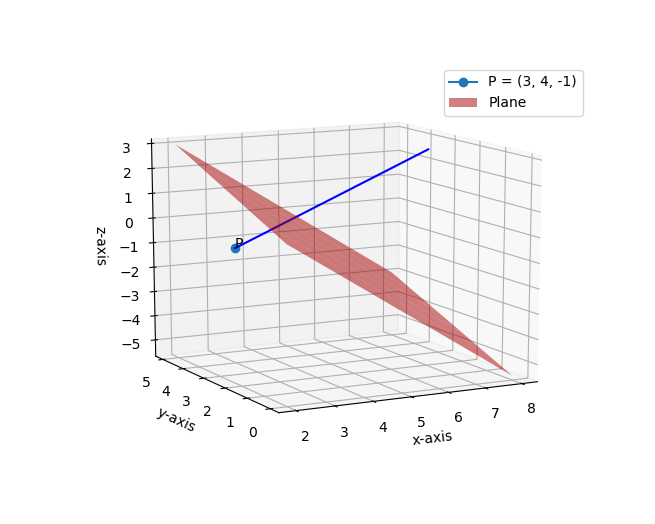
\includegraphics[width = \columnwidth]{assignment_8.png}
    \caption{Line passing through $\myvec{3 & 4 & -1}$ and perpendicular to the plane $2x - y + 2z = 5$.}
    \label{line and plane}
\end{figure}
\end{document}
